\documentclass[11pt]{article}
\usepackage[scaled=0.92]{helvet}
\usepackage{geometry}
\geometry{letterpaper,tmargin=1in,bmargin=1in,lmargin=1in,rmargin=1in}
\usepackage[parfill]{parskip} % Activate to begin paragraphs with an empty line rather than an indent %\usepackage{graphicx}
\usepackage{amsmath,amssymb, mathrsfs,  mathtools, dsfont}
\usepackage{tabularx}
\usepackage{tikz-cd}
\usepackage[font=footnotesize,labelfont=bf]{caption}
\usepackage{graphicx}
\usepackage{xcolor}
%\usepackage[linkbordercolor ={1 1 1} ]{hyperref}
%\usepackage[sf]{titlesec}
\usepackage{natbib}
\usepackage{../../Tianpei_Report}


\begin{document}
\title{Lecture 7: Complete Metric Spaces and Function Spaces}
\author{ Tianpei Xie}
\date{ Nov. 30th., 2022 }
\maketitle
\tableofcontents
\newpage
\section{Complete Metric Space}
\begin{itemize}
\item \begin{definition} (\emph{\textbf{Cauchy Net in Topological Vector Space}})\\
A \emph{net}  $\set{x_\alpha}_{\alpha \in I}$ in \emph{\textbf{toplogocial vector space}} $X$ is called \underline{\emph{\textbf{Cauchy}}} if the net $\set{x_{\alpha} - x_{\beta}}_{(\alpha, \beta) \in I \times I}$
\emph{\textbf{converges} to zero}. (Here $I \times I$ is \emph{\textbf{directed}} in the usual way: $(\alpha, \beta) \prec (\alpha', \beta')$ if and only if $\alpha \prec \alpha'$ and $\beta \prec \beta'$.) 
\end{definition}

\item \begin{definition} (\emph{\textbf{Completeness}})\\
A toplogocial vector space $X$ is \emph{\textbf{complete}} if every Cauchy net converges.
\end{definition}

\item \begin{proposition} (\textbf{Complete First Countable Topological Vector Space})\\
If $X$ is a \textbf{first-countable topological vector space} and every \textbf{Cauchy sequence} in $X$ converges, then every \textbf{Cauchy net} in $X$ converges.
\end{proposition}

\item \begin{proposition} (\textbf{Completeness of Euclidean Space}) \citep{munkres2000topology} \\
Euclidean space $\bR^k$ is \textbf{complete} in either of its usual \textbf{metrics}, the \textbf{euclidean metric} $d$ or the \textbf{square metric} $\rho$.
\end{proposition}

\item \begin{lemma} (\textbf{Convergence in Product Space is Weak Convergence}) \citep{munkres2000topology} \\
Let $X$ be the product space $X = \prod_{\alpha}X_{\alpha}$; let $x_n$ be a sequence of points of $X$. Then $x_n \rightarrow x$ if and only if $\pi_{\alpha}(x_n) \rightarrow  \pi_{\alpha}(x)$ for each $\alpha$.
\end{lemma}

\item \begin{proposition} (\textbf{Completeness of Countable Product Space}) \citep{munkres2000topology} \\
There is a metric for the product space $\bR^{\omega}$ relative to which $\bR^{\omega}$ is \textbf{complete}.
\end{proposition}

\item \begin{definition} (\emph{\textbf{Uniform Metric in Function Space}})\\
Let $(Y, d)$ be a metric space; let $\bar{d}(a, b) = \min\{d(a, b), 1\}$ be the \emph{\textbf{standard bounded metric}} on $Y$ derived from $d$. If $x = (x_{\alpha})_{\alpha \in J}$ and  $y = (y_{\alpha})_{\alpha \in J}$ are points of the cartesian product $Y^J$, let
\begin{align*}
\bar{\rho}(x, y) = \sup\set{\bar{d}(x_{\alpha}, y_{\alpha}): \alpha \in J}.
\end{align*}
It is easy to check that $\bar{\rho}$ is a metric; it is called \underline{\emph{\textbf{the uniform metric}}} on $Y^J$ corresponding to the metric $d$ on $Y$.

Note that \emph{\textbf{the space of all functions} $f: J \rightarrow Y$}, \emph{\textbf{denoted}} as $Y^{J}$, is a subset of the product space $J \times Y$. We can define uniform metric in the function space: if $f$, $g : J \rightarrow Y$, then
\begin{align*}
\bar{\rho}(f, g) = \sup\set{\bar{d}(f(\alpha), g(\alpha)): \alpha \in J}.
\end{align*}
\end{definition}

\item \begin{proposition} (\textbf{Completeness of Function Space  Under Uniform Metric}) \citep{munkres2000topology} \\
If the space $Y$ is \textbf{complete} in the metric $d$, then the space $Y^J$ is \textbf{complete} in the \textbf{uniform metric} $\bar{\rho}$ corresponding to $d$.
\end{proposition}

\item \begin{definition} (\emph{\textbf{Space of Continuous Functions and Bounded Functions}})\\
Let $Y^{X}$ be  \emph{the space of all functions} $f: X \rightarrow Y$, where $X$ is a \emph{topological space} and $Y$ is a \emph{metric space with metric $d$}. Denote the \emph{\textbf{subspace}}  of $Y^X$ consisting of all \emph{\textbf{continuous functions} $f$} as $\cC(X, Y)$. 

Also denote \emph{the set  of all \textbf{bounded functions}} $f: X \rightarrow Y$ as $\cB(X, Y)$. (A function $f$ is said to be \emph{\textbf{bounded}} if its image $f(X)$ is a \emph{\textbf{bounded subset}} of \emph{the metric space $(Y, d)$}.) 
\end{definition}

\item \begin{proposition}  (\textbf{Completeness of $\cC(X, Y)$ and   $\cB(X, Y)$  Under Uniform Metric}) \citep{munkres2000topology} \\
Let $X$ be a topological space and let $(Y, d)$ be a metric space. The set $\cC(X, Y)$ of \textbf{continuous} functions is \textbf{closed} in $Y^X$ under the \textbf{uniform metric}. So is the set $\cB(X, Y)$ of \textbf{bounded functions}. Therefore, if $Y$ is \textbf{complete}, these spaces are \textbf{complete} in the \textbf{uniform metric}.
\end{proposition}

\item \begin{definition} (\emph{\textbf{Sup Metric on Bounded Functions}})\\
If $(Y, d)$ is a metric space, one can define another metric \emph{on the set $\cB(X, Y)$ of \textbf{bounded functions}} from $X$ to $Y$ by the equation
\begin{align*}
\rho(x, y) = \sup\set{d(f(x), g(x)): x \in X}.
\end{align*}
It is easy to see that $\rho$ is well-defined, for the set $f(X) \cup g(X)$ is \emph{\textbf{bounded}} if both $f(X)$ and $g(X)$ are. The metric $\rho$ is called \underline{\emph{\textbf{the sup metric}}}.
\end{definition}

\item \begin{theorem} (\textbf{Existence of Completion}) \citep{munkres2000topology}\\
Let $(X, d)$ be a metric space. There is an \textbf{isometric embedding} of $X$ into a \textbf{complete} metric space.
\end{theorem}

\item \begin{definition} (\emph{\textbf{Completion}})\\
Let $X$ be a \emph{metric space}. If $h : X \rightarrow Y$ is an \textbf{\emph{isometric embedding}} of $X$ into a \emph{\textbf{complete} metric space} $Y$, then the \emph{\textbf{subspace}} $h(X)$ of $Y$ is a \emph{complete metric space}. It is called \underline{\emph{\textbf{the completion of $X$}}}.
\end{definition}

\item \begin{definition} (\emph{\textbf{Topological Complete}})\\
A space $X$ is said to be \underline{\emph{\textbf{topologically complete}}} if there \emph{exists} a metric for the \emph{topology} of $X$ relative to which $X$ is \emph{complete}.
\end{definition}

\item \begin{proposition} (\textbf{Properties of Topological Complete}) \citep{munkres2000topology}\\
The followings are properties of topological completeness:
\begin{enumerate}
\item A \textbf{closed} subspace of a topologically complete space is topologically complete.
\item A \textbf{countable product} of topologically complete spaces is topologically complete (in the \textbf{product topology}).
\item An \textbf{open} subspace of a topologically complete space is topologically complete.
\item A \textbf{$G_{\delta}$ set} in a topologically complete space is topologically complete. 
\end{enumerate}
\end{proposition}
\end{itemize}

\section{Compactness in Metric Spaces}
\subsection{Total Boundedness and Equicontinuous}
\begin{itemize}
\item \begin{remark} (\emph{Relate \textbf{Compactness} to \textbf{Completeness}})\\
How is \emph{\textbf{compactness}} of a metric space $X$ related to \emph{\textbf{completeness}} of $X$? 

The followings is from \emph{the sequential compactness} and definition of \emph{completeness}:
\begin{proposition}
Every \textbf{compact} metric space is \textbf{complete}.
\end{proposition}
The \emph{converse} does not hold -- \emph{\textbf{a complete metric space need not be compact}}. It is reasonable to ask what \emph{\textbf{extra condition}} one needs to impose on a complete space to be assured of its compactness.
Such a condition is the one called \emph{total boundedness}.
\end{remark}

\item \begin{definition} (\emph{\textbf{Total Boundedness}})\\
A metric space $(X, d)$ is said to be \underline{\emph{\textbf{totally bounded}}} if for every $\epsilon > 0$, there is a \emph{\textbf{finite covering} of $X$ by \textbf{$\epsilon$-balls}}.
\end{definition}

\item \begin{theorem} (\textbf{Total Boundedness  $+$ Completeness $=$ Compactness})\citep{munkres2000topology}\\
A metric space $(X, d)$ is \underline{\textbf{compact}} \textbf{if and only if} it is \underline{\textbf{complete}} and \underline{\textbf{totally bounded}}.
\end{theorem}

\item \begin{remark}
We now apply this result to find \emph{\textbf{the compact subspaces}} of the space $\cC(X, \bR^n)$, \emph{in the \textbf{uniform topology}}. We know that a subspace of $\bR^n$ is compact if and only if it is \emph{\textbf{closed}} and \emph{\textbf{bounded}}. 

One might hope that an analogous result holds for $\cC(X, \bR^n)$. \emph{\textbf{But}} it does not, even if $X$ is \emph{compact}. One needs to assume that the subspace of $\cC(X, \bR^n)$ satisfies \emph{an \textbf{additional condition}}, called \emph{\textbf{equicontinuity}}. 
\end{remark}

\item \begin{definition}  (\emph{\textbf{Equicontinuity}}) \citep{reed1980methods, munkres2000topology} \\
Let $(Y, d)$ be a \emph{metric space}. Let $\srF$ be a \emph{subset} of the function space $\cC(X, Y)$ (i.e. $f \in \srF$ is continuous). If $x_0 \in X$, \emph{the set $\srF$ of functions} is said to be \underline{\emph{\textbf{equicontinuous at $x_0$}}} if given $\epsilon >0$, there is a neighborhood $U$ of $x_0$ such that \emph{for all $x \in U$} and \underline{\emph{\textbf{all $f \in \srF$}}},
\begin{align*}
d(f(x), f(x_0)) < \epsilon.
\end{align*}
If the set $\srF$ is \emph{equicontinuous} at $x_0$ for each $x_0 \in X$, it is said simply to be \underline{\emph{\textbf{equicontinuous}}} or $\srF$ is an \underline{\emph{\textbf{equicontinuous family}}}.

We say $\srF$ is a \underline{\emph{\textbf{uniformly equicontinuous family}}} if and only if for all $\epsilon >0$, there exists $\delta > 0$ such that $d(f(x), f(x')) < \epsilon$ whenever $p(x, x') < \delta$ for all $x, x' \in X$ and \emph{\textbf{every $f \in \srF$}}.
\end{definition}

\item \begin{remark}
An \emph{equicontinuous family} of functions is \emph{a family of continuous functions}.
\end{remark}

\item \begin{remark}
\emph{\textbf{Continuity}} of the function $f$ at $x_0$ means that \emph{\textbf{given} $f$} and given $\epsilon >0$, there exists a neighborhood $U$ of $x_0$ such that $d(f(x), f(x_0)) < \epsilon$ for $x \in U$. 
\textbf{
\emph{\textbf{Equicontinuity}} of $\srF$ means that \emph{\textbf{a single neighborhood}} $U$ can be chosen that will \emph{}work for all the functions} $f$ in the collection $\srF$.
\end{remark}

\item \begin{lemma} (\textbf{Total Boundedness $\Rightarrow$ Equicontinuous}) \citep{munkres2000topology}\\ 
Let $X$ be a \textbf{space}; let $(Y, d)$ be a \textbf{metric} space. If the subset $\srF$ of $\cC(X, Y)$ is \textbf{totally bounded} under the \textbf{uniform metric} corresponding to $d$, then $\srF$ is \textbf{equicontinuous} under $d$.
\end{lemma}

\item \begin{lemma} (\textbf{Equicontinuous $+$ Compactness  $\Rightarrow$ Total Boundedness})  \citep{munkres2000topology}\\ 
Let $X$ be a space; let $(Y, d)$ be a metric space; assume $X$ and $Y$ are \textbf{compact}. If the subset $\srF$ of $\cC(X, Y)$ is \textbf{equicontinuous} under $d$, then $\srF$ is \textbf{totally bounded} under the \textbf{uniform} and \textbf{sup} metrics corresponding to $d$.
\end{lemma}


%\item \begin{proposition}
%Let $f_n$ be a sequence of functions from one metric space to another with the property that the family $\{f_n\}$ is \textbf{equicontinuous}. Suppose
%that $f_n(x) \rightarrow f(x)$ \textbf{pointwise} for each $x$. Then $f$ is \textbf{continuous}.
%\end{proposition}
%
%\item We see that \emph{\textbf{pointwise convergence}} on a \emph{\textbf{dense set}} combined with \emph{\textbf{equicontinuity}} implies \emph{\textbf{pointwise convergence everywhere}}.
%\begin{proposition} \citep{reed1980methods}\\
%Let $\{f_n\}$ be an \textbf{equicontinuous family} of functions from one metric space $(X, p)$ to another $(Y, d)$ with $Y$ complete. Suppose that for a \textbf{dense} set $D \subseteq X$, we know $f_{n}(x)$ converges for all $x \in D$. Then $f_{n}(x)$ converges for all $x \in X$.
%\end{proposition}
%
%\item The following shows that uniformly equicontinuous combined with pointwise convergence implies uniform convergence.
%\begin{proposition} \citep{reed1980methods}\\
%Let $\{f_n\}$ be a \textbf{uniformly equicontinuous family} of functions on $[0, 1]$. Suppose that $f_n(x) \rightarrow f(x)$ for each $x$ in $[0, 1]$. Then $f_n(x) \rightarrow f(x)$  \textbf{uniformly} in $x$.
%\end{proposition}
%
%\item \begin{remark}
%For functions on $[0, 1]$, \emph{every \textbf{equicontinuous family}} is \emph{\textbf{uniformly equicontinuous}}.
%\end{remark}

\item \begin{definition} (\emph{\textbf{Pointwise Bounded}})\\
If $(Y, d)$ is a \emph{metric space}, a \emph{subset} $\srF$ of $\cC(X, Y)$ is said to be \underline{\emph{\textbf{pointwise bounded}}} under $d$ if for each $x \in X$, the subset
\begin{align*}
F_{a} &= \set{f(a): f\in \srF}
\end{align*}
of $Y$ is \emph{\textbf{bounded}} under $d$.
\end{definition}

\item \begin{theorem} (\textbf{Ascoli's Theorem, Classical Version}). \citep{munkres2000topology}\\
Let $X$ be a \underline{\textbf{compact} space}; let $(\bR^n , d)$ denote euclidean space in either the square metric or the euclidean metric; give $\cC(X, \bR^n)$ the corresponding \textbf{uniform topology}. A subspace $\srF$ of $\cC(X, \bR^n)$ has \underline{\textbf{compact closure}} \textbf{if and only if} $\srF$ is \underline{\textbf{equicontinuous}} and \underline{\textbf{pointwise bounded}} under $d$.
\end{theorem}



\item \begin{corollary}\citep{munkres2000topology}\\
Let $X$  be  \underline{\textbf{compact}}; let $d$ denote either the square metric or the euclidean metric on $\bR^n$; give $\cC(X, \bR^n)$ the corresponding \textbf{uniform topology}. A subspace $\srF$ of $\cC(X, \bR^n)$ is \underline{\textbf{compact}} \textbf{if and only if} it is \underline{\textbf{closed}, \textbf{bounded}} under the \underline{\textbf{sup metric} $\rho$}, and \textbf{equicontinuous} under $d$.
\end{corollary}

\item \begin{corollary} (\textbf{Ascoli's Theorem, Sequence Version}) \citep{reed1980methods}\\
Let $\{f_n\}$ be a family of \textbf{uniformly bounded equicontinuous functions} on $[0, 1]$. Then \textbf{some subsequence} $\{f_{n,m}\}$ converges \textbf{uniformly} on $[0, 1]$.
\end{corollary}

\item \begin{definition} (\emph{\textbf{Continuous Functions that Vanish At Infinity $\cC_0(X, \bR)$}}) \\
Let $X$ be a space. A subset $\cF$ of $\cC(X, \bR)$ is said to \underline{\emph{\textbf{vanish uniformly at infinity}}} if given $\epsilon > 0$, there is a \emph{\textbf{compact subspace}} $C$ of $X$ such that $\abs{f(x)} < \epsilon$  for $x \in X \setminus C$ and $f \in \cF$. 

If $\cF$ consists of a single function $f$, we say simply that \underline{\emph{\textbf{$f$ vanishes at infinity}}}. Let $\cC_0(X, \bR)$ denote \emph{the set of continuous functions $f : X \rightarrow \bR$ that \textbf{vanish at infinity}}.
\end{definition}

\item \begin{corollary} \citep{munkres2000topology}\\
Let $X$ be \underline{\textbf{locally compact Hausdorff}}; give $\cC_0(X, \bR)$ the uniform topology. A subset $\cF$ of $\cC_0(X, \bR)$ has \underline{\textbf{compact closure}}  \textbf{if and only if} it is \underline{\textbf{pointwise bounded}}, \underline{\textbf{equicontinuous}}, and \underline{\textbf{vanishes uniformly at infinity}}.
\end{corollary}
\end{itemize}

\subsection{Pointwise and Compact Convergence}
\begin{itemize}
\item \begin{definition} (\emph{\textbf{Topology of Pointwise Convergence / Point-Open Topology}})\\
Given a point $x$ of the set $X$ and an open set $U$ of the space $Y$, let
\begin{align*}
S(x, U) = \set{f:  f \in Y^X\text{ and }f(x) \in U}.
\end{align*}
The sets $S(x, U)$ are a \emph{\textbf{subbasis}} for \emph{topology} on $Y^X$, which is called \underline{\emph{\textbf{the topology}}} of \underline{\emph{\textbf{pointwise convergence}}} (or \underline{\emph{\textbf{the point-open topology}}})
\end{definition}



\begin{figure}
\begin{minipage}[t]{1\linewidth}
  \centering
  \centerline{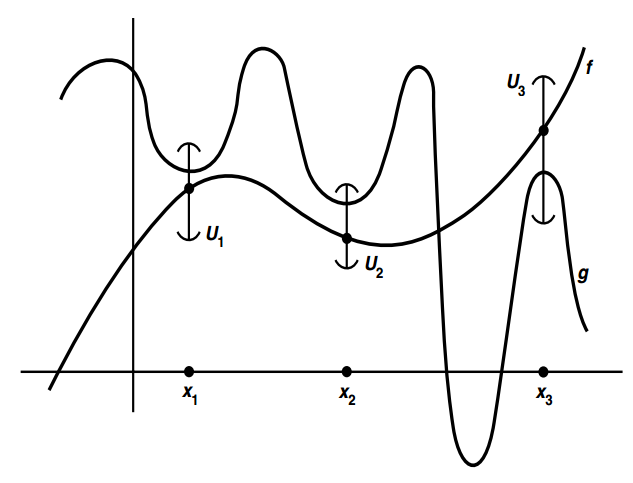
\includegraphics[scale = 0.4]{pointwise_convergence_topology.png}}
\end{minipage}
\caption{\footnotesize{\textbf{The function $g$ in neighborhood of $f$ in topology of pointwise convergence. \citep{munkres2000topology}}}}
\label{fig: pointwise_convergence_topology}
\end{figure}


\item \begin{remark} (\emph{\textbf{Basis of Point-Open Topology}})\\
The general \emph{basis element} for this topology is a \emph{finite intersection} of subbasis elements $S(x, U)$. Thus a typical \emph{\textbf{basis element}} about the function $f$ \emph{consists of all functions $g$ that are \underline{\textbf{``close"} to $f$ \textbf{at finitely many points}}}. Such a \emph{neighborhood} is illustrated in Figure \ref{fig: pointwise_convergence_topology}; it consists of all functions $g$ whose graphs \emph{intersect the three vertical intervals} pictured.
\end{remark}

\item \begin{remark}
\emph{\textbf{The topology of pointwise convergence on $Y^X$ is \underline{the product topology}}}. 

If we replace $X$ by $J$ and denote the general element of $J$ by $\alpha$ to make it look more familiar, then the set $S(\alpha, U)$ of all functions $x : J \rightarrow Y$
such that $x(\alpha) \in U$ is just the subset $\pi_{\alpha}^{-1}(U)$ of $Y^J$, which is \emph{the standard subbasis element} for the product topology.
\end{remark}

\item \begin{proposition} (\textbf{Pointwise Convergence Topology})\citep{munkres2000topology}\\
A sequence $f_n$ of functions \textbf{converges} to the function $f$ in the \textbf{topology of pointwise convergence} \textbf{if and only if} for \textbf{each} $x$ in $X$, the sequence $f_n(x)$ of \textbf{points of $Y$} converges to the point $f(x)$.
\end{proposition}


\item \begin{remark}
Compare the \emph{subbasis} of \emph{the point-open topology} on function space $Y^X$ and \emph{the weak topology} on space $X$
\begin{align*}
S(x, U) = \set{f:  f \in Y^X\text{ and }f(x) \in U} &\quad \text{\emph{point-open topology}}.\\
B(f, U) = \set{x:  x \in X\text{ and }f(x) \in U} &\quad \text{\emph{weak topology}}.
\end{align*}
\end{remark}

\item \begin{example} (\textbf{\emph{Pointwise Convergence Does Not Preserve Continuity}})\\
Consider the space $\bR^I$, where $I = [0, 1]$. The sequence $(f_n)$ of continuous functions given by $f_n(x) = x^n$ \emph{converges} in the \emph{\textbf{topology of pointwise convergence}} to the function $f$ defined by
\begin{align*}
f(x) &=\left\{ 
\begin{array}{cc}
0 &\text{ for } 0 \le x < 1\\
1 &\text{ for } x = 1
\end{array}\right.,
\end{align*}
This example shows that the subspace $\cC(I, \bR)$ of continuous functions is \emph{\textbf{not closed}} in $\bR^I$
\emph{in the topology of pointwise convergence}. Note that $\cC(I, \bR)$  is \emph{\textbf{closed} in $\bR^I$ under \textbf{uniform topology}} due to \emph{Uniform Limit theorem}. 
\end{example}

\item \begin{definition} (\emph{\textbf{Topology of Compact Convergence}})\\
Let $(Y, d)$ be a \emph{metric space}; let $X$ be a \emph{topological space}. Given an element $f$ of $Y^X$, a \emph{\textbf{compact subspace}} $C$ of $X$, and a number $\epsilon > 0$, let $B_{C}(f, \epsilon)$ denote the set of all those elements $g$ of $Y^X$ for which
\begin{align*}
\sup\{d(f (x), g(x)): x \in C\} < \epsilon.
\end{align*}
The sets $B_{C}(f, \epsilon)$  form a \emph{\textbf{basis}} for a topology on $Y^X$. It is called the \underline{\emph{\textbf{topology of compact}}} \underline{\emph{\textbf{convergence}}} (or sometimes the ``\underline{\emph{\textbf{topology of uniform convergence on compact sets}}}").
\end{definition}

\item \begin{proposition} (\textbf{Topology of Uniform Convergence in Compact Sets}) \citep{munkres2000topology}\\
A sequence $f_n : X \rightarrow Y$ of functions converges to the function $f$ in the \textbf{topology of compact convergence} if and only if for \textbf{each compact subspace} $C$ of $X$, the sequence $f_n|_{C}$ converges \textbf{uniformly} to $f|_C$.
\end{proposition}

\item \begin{definition} (\emph{\textbf{Compactly Generated Space}})\\
A space $X$ is said to be \underline{\emph{\textbf{compactly generated}}} if it satisfies the following condition: A set $A$ is \emph{\textbf{open (or closed)}} in $X$ if $A \cap C$ is \emph{\textbf{open (or closed)}} in $C$ for each \textbf{\emph{compact subspace}} $C$ of $X$.
\end{definition}

\item \begin{lemma} \citep{munkres2000topology}\\
If $X$ is \textbf{locally compact}, or if $X$ satisfies \textbf{the first countability axiom}, then $X$ is \textbf{compactly generated}.
\end{lemma}

\item The crucial fact about compactly generated spaces is the following:
\begin{lemma} (\textbf{Continuous Extension on Compact Generated Space})  \citep{munkres2000topology}\\
If $X$ is compactly generated, then a function $f : X \rightarrow Y$ is \textbf{continuous} if for each \textbf{compact subspace} $C$ of X, the restricted function $f |_{C}$ is \textbf{continuous}.
\end{lemma}
\begin{proof}
Let $V$ be an \emph{open} subset of $Y$; we show that $f^{-1}(V)$ is \emph{open} in $X$. Given any subspace $C$ of $X$,
\begin{align*}
f^{-1}(V) \cap C = (f|_C)^{-1}(V).
\end{align*}
If $C$ is \emph{compact}, this set is \emph{open} in $C$ because $f|_C$ is \emph{continuous}. Since $X$ is \emph{compactly generated}, it follows that $f^{-1}(V)$ is \emph{open} in $X$. \qed
\end{proof}

\item \begin{theorem} (\textbf{$\cC(X, Y)$ on Compact Generated Space})  \citep{munkres2000topology}\\
Let $X$ be a \underline{\textbf{compactly generated space}}: let $(Y, d)$ be a metric space. Then $\cC(X, Y)$ is \underline{\textbf{closed}} in $Y^X$ in the \underline{\textbf{topology of compact convergence}}.
\end{theorem}
\begin{proof}
Let $f \in Y^X$ be a \emph{limit point} of $\cC(X, Y)$; we wish to show $f$ is \emph{continuous}.

It suffices to show that $f|_C$ is \emph{continuous} for each \emph{compact subspace} $C$ of $X$, since by lemma above, we can extend $f$ on entire space. For each $n$, consider the \emph{neighborhood} $B_C(f, 1/n)$ of $f$; it \emph{intersects} $\cC(X, Y)$, so we can choose a function $f_n \in \cC(X, Y)$ lying in this neighborhood. The sequence of functions $f_n|_{C}: C \rightarrow Y$ \emph{converges uniformly} to the function $f|_C$, so that by \emph{the uniform limit theorem}, $f|_C$ is \emph{continuous}. \qed
\end{proof}

\item \begin{corollary} (\textbf{Compact Convergence Limit})  \citep{munkres2000topology}\\
Let $X$ be a \textbf{compactly generated space}; let $(Y, d)$ be a \textbf{metric} space. If a sequence of \textbf{continuous} functions $f_n : X \rightarrow Y$ converges to $f$ in the \textbf{topology of compact convergence}, then $f$ is \textbf{continuous}.
\end{corollary}

\item \begin{remark} (\emph{\textbf{Useful Topologies on $Y^X$}})
\begin{enumerate}
\item \underline{\emph{\textbf{Uniform Topology}}}: generated by the \emph{\textbf{basis}}
\begin{align*}
B_{U}(f, \epsilon) &= \set{g \in Y^X: \sup_{x\in X}\bar{d}(f(x), g(x)) < \epsilon }
\end{align*} It corresponds to \emph{\textbf{the uniform convergence}} of $f_n$ to $f$ in $Y^X$. $\cC(X, Y)$ is \emph{\textbf{closed}} in $Y^X$ under the \emph{uniform topology}, following \emph{the Uniform Limit Theorem}.

\item  \underline{\emph{\textbf{Topology of Pointwise Convergence}}}: generated by the \emph{\textbf{basis}}
\begin{align*}
B_{U_1 \xdotx{,} U_n}(x_1 \xdotx{,} x_n, \epsilon)  &= \bigcap_{i=1}^{n}S(x_i, U_i) \\
&= \set{f \in Y^X: f(x_1) \in U_1 \xdotx{,} f(x_n) \in U_n}, \quad   1 \le n < \infty.
\end{align*} It corresponds to \emph{\textbf{the pointwise convergence}} of $f_n$ to $f$ in $Y^X$. $\cC(X, Y)$ is \emph{\textbf{not closed}} in $Y^X$ under the \emph{topology of pointwise convergence}

\item \underline{\emph{\textbf{Topology of Compact Convergence}}}: generated by the \emph{\textbf{basis}}
\begin{align*}
B_{C}(f, \epsilon) &= \set{g \in Y^X: \sup_{x \in C}d(f (x), g(x)) < \epsilon }.
\end{align*} It corresponds to \emph{\textbf{the uniform convergence}} of $f_n$ to $f$ in $Y^X$ for $x \in C$. $\cC(X, Y)$ is \emph{\textbf{closed}} in $Y^X$ under the \emph{topology of compact convergence} \emph{\textbf{if $X$ is compactly generated}}.
\end{enumerate}
\end{remark}

\item \begin{theorem} (\textbf{Relationship between Topologies on $Y^X$}) \citep{munkres2000topology}\\
Let $X$ be a space; let $(Y, d)$ be a metric space. For the function space $Y^X$ , one has the following \textbf{inclusions of topologies}:
\begin{align*}
\text{\textbf{(uniform)}} \supseteq \text{\textbf{(compact convergence)}} \supseteq \text{\textbf{(pointwise convergence)}}.
\end{align*}
If $X$ is \textbf{compact}, the \textbf{first two} coincide, and if $X$ is \textbf{discrete}, the \textbf{second two} coincide.
\end{theorem}

\item \begin{remark}
Note that both \emph{uniform topology} and \emph{topology of compact convergence} rmade specific use of the metric $d$ for the space $Y$, i.e. it can only be defined when the image of function $Y$  is a metric space.

But \emph{\textbf{the topology of  pointwise convergence}} does \emph{not use the definition of metric} $d$ in $Y$. In fact, \emph{\textbf{it is defined for any image space $Y$}}.
\end{remark}

\item \begin{definition} (\emph{\textbf{Compact-Open Topology on Continuous Function Space}})\\
Let $X$ and $Y$ be topological spaces. If $C$ is a \emph{\textbf{compact subspace}} of $X$ and $U$ is an \emph{open} subset of $Y$, define
\begin{align*}
S(C,U) = \set{ f \in \cC(X, Y): f(C) \subseteq U}.
\end{align*}
The sets $S(C, U)$ form a \emph{\textbf{subbasis}} for a \emph{topology} on $\cC(X, Y)$ that is called \underline{\emph{\textbf{the compact-open}}} \underline{\emph{\textbf{topology}}}.
\end{definition}

\item \begin{proposition} (\textbf{Compact-Open on $\cC(X, Y)$ $=$ Compact Convergence}) \citep{munkres2000topology}\\
Let $X$ be a space and let $(Y, d)$ be a metric space. On the set $\cC(X, Y)$, the \textbf{compact-open topology} and the \textbf{topology of compact convergence} \textbf{coincide}.
\end{proposition}

\item \begin{corollary}(\textbf{Compact Convergence on $\cC(X, Y)$ Need Not $d$}) \citep{munkres2000topology}\\
Let $Y$ be a metric space. The \textbf{compact convergence topology} on $\cC(X, Y)$ does  \textbf{not} depend on the \textbf{metric} of $Y$. Therefore if $X$ is \textbf{compact}, the \textbf{uniform topology} on $\cC(X, Y)$ does not depend on the metric of $Y$.
\end{corollary}

\item \begin{remark} 
The fact that the definition of \emph{\textbf{the compact-open topology}} does not involve a \emph{\textbf{metric}} is just one of its useful features. 

Another is the fact that it satisfies the requirement of ``\emph{\textbf{joint continuity}}.” Roughly speaking, this means that the expression $f(x)$ is
\emph{continuous} not only in the \emph{single}``variable”  $x$, but is \emph{\textbf{continuous jointly} in \textbf{both} the $x$ and $f$} .
\end{remark}

\item \begin{theorem} (\textbf{Compact-Open Topology $\Rightarrow$ Joint Continuity for $x$ and $f$})\\
Let $X$ be \textbf{locally compact Hausdorff}; let $\cC(X, Y)$ have the \textbf{compact-open topology}. Then the map
\begin{align*}
e: X \times \cC(X, Y) \rightarrow Y
\end{align*}
defined by the equation
\begin{align*}
e(x, f) = f(x)
\end{align*}
is \textbf{continuous}. The map $e$ is called \underline{\textbf{the evaluation map}}.
\end{theorem}

\item \begin{definition}
Given a function $f : X \times Z \rightarrow Y$, there is a corresponding function $F : Z \rightarrow \cC(X, Y)$, defined by the equation
\begin{align*}
(F(z))(x) = f(x, z).
\end{align*}
Conversely, given $F : Z \rightarrow \cC(X, Y)$, this equation defines a corresponding function
$f : X \times Z \rightarrow Y$. We say that $F$ is the map of $Z$ into $\cC(X, Y)$ that is induced by $f$.
\end{definition}

\item \begin{proposition}
Let $X$ and $Y$ be spaces; give $\cC(X, Y)$ the \textbf{compact-open topology}. If $f: X \times Z \rightarrow Y$ is \textbf{continuous}, then \textbf{so is} the induced function $F : Z \rightarrow \cC(X, Y)$. The \textbf{converse} holds if $X$ is \textbf{locally compact Hausdorff}.
\end{proposition}
\end{itemize}

\subsection{Ascoli's Theorem}
\begin{itemize}
\item \begin{theorem} (\textbf{Ascoli's Theorem, General Version}). \citep{munkres2000topology} \\
Let $X$ be a space and let $(Y, d)$ be a \underline{\textbf{metric}} space. Give $\cC(X, Y)$ the \underline{\textbf{topology of compact}} \underline{\textbf{convergence}}; let $\cF$ be a subset of $\cC(X, Y)$.
\begin{enumerate}
\item If $\cF$ is \underline{\textbf{equicontinuous}} under $d$ and the set
\begin{align*}
F_{a} &= \set{f(a): f \in \cF}
\end{align*}
has \underline{\textbf{compact closure}} for each $a \in X$, then $\cF$ is \underline{\textbf{contained} in a \textbf{compact subspace}} of $\cC(X, Y)$.
\item  The \textbf{converse} holds if $X$ is \underline{\textbf{locally compact Hausdorff}}.
\end{enumerate}
\end{theorem}

\item \begin{remark} 
Compare with classical version, we see generalizations:
\begin{enumerate}
\item $X$ need not to be \emph{\textbf{compact}}; $\Rightarrow$ does not even need $X$ to be topological. $\Leftarrow$ holds when $X$ is \textbf{\emph{locally compact Hausdorff}}.
\item $\cC(X, Y)$ is under \emph{\textbf{compact-open topology}} which is \emph{\textbf{weaker}} than \emph{\textbf{uniform topology}}, i.e. we does not require convergence of sequence \emph{uniformly} but only \emph{uniformly in a compact subset}.
\item $\cF$ does not need to be \emph{\textbf{pointwise bounded}} under $d$. In other word, the set 
\begin{align*}
F_{a} &= \set{f(a): f \in \cF}
\end{align*} need not to be \emph{\textbf{bounded}} but need to have \emph{\textbf{compact closure}} for each $a \in X$. Note that for metric space $Y$, if $Y$ is finite dimensional, it is the same requirement as boundness. But compact closure is stronger than bounded.
\end{enumerate}
\end{remark}

\item \begin{proposition} (\textbf{Equicontinuity $+$ Pointwise Convergence $\Rightarrow$ Compact Convergence}) \citep{munkres2000topology}\\
Let $(Y, d)$ be a metric space; let $f_n : X \rightarrow Y$ be a sequence of \textbf{continuous} functions; let $f : X \rightarrow Y$ be a function (not necessarily continuous). Suppose $f_n$ converges to $f$ in the \textbf{topology of pointwise convergence}. If $\{f_n\}$ is \textbf{equicontinuous}, then $f$ is \textbf{continuous} and $f_n$ converges to $f$ in the \textbf{topology of compact convergence}.
\end{proposition}
\end{itemize}

\section{Baire Category Theorem}
\begin{itemize}
\item \begin{remark} (\emph{\textbf{Empty Interior $=$ Complement is Dense}}) \\
Recall that if $A$ is a subset of a space $X$, the \emph{\textbf{interior}} of $A$ is defined as \emph{the union of all open sets of $X$ that are contained in $A$}. 

To say that $A$ has \underline{\emph{\textbf{empty interior}}} is to say then that \emph{\textbf{$A$ \underline{contains no open set} of $X$} other than the empty set}. \emph{\textbf{Equivalently}}, $A$ has \emph{\textbf{empty interior}} if every point of $A$ is \emph{a \textbf{limit point} of the \textbf{complement} of $A$}, that is, if \underline{\emph{the \textbf{complement} of $A$ is \textbf{dense} in $X$}}.
\begin{align*}
\mathring{A} = \emptyset \;\; \Leftrightarrow \;\; A^{c}\text{ is dense in }X
\end{align*} In \citep{reed1980methods}, if a subset $\overline{A}$ of $X$ has \emph{empty interior}, $A$ is said to be \underline{\emph{\textbf{nowhere dense}}} in $X$.
\end{remark}

\item \begin{example} 
Some  examples:
\begin{enumerate}
\item The set $\bQ$ of \emph{rationals} has \emph{\textbf{empty interior}} as a subset of $\bR$
\item The \emph{interval} $[0, 1]$ has \emph{\textbf{nonempty interior}}. 
\item The \emph{interval} $[0, 1] \times 0$ has \emph{\textbf{empty interior}} as a \emph{subset of the plane} $\bR^2$, and so does the \emph{subset} $\bQ \times \bR$.
\end{enumerate}
\end{example}

\item \begin{definition} (\emph{\textbf{Baire Space}})\\
A space $X$ is said to be a \underline{\emph{\textbf{Baire space}}} if the following condition holds:  Given  \emph{\textbf{any countable}} collection $\set{A_n}$ of \emph{\textbf{closed}} sets of $X$ each of which has \emph{\textbf{empty interior}} in $X$, their \emph{\textbf{union}}  $\bigcup_{n=1}^{\infty} A_n$ also has \emph{\textbf{empty interior}} in $X$.
\end{definition}

\item \begin{example} 
Some  examples:
\begin{enumerate}
\item The space $\bQ$ of \emph{rationals} is \emph{\textbf{not} a \textbf{Baire space}}. For each one-point set in $\bQ$ is \emph{closed and has empty interior \textbf{in $\bQ$}}; and $\bQ$ is \emph{the countable union of its one-point subsets}.
\item The space $\bZ_{+}$, on the other hand, does form \emph{a \textbf{Baire space}}. Every subset of $\bZ_{+}$ is \emph{open}, so that there exist \emph{no subsets} of $\bZ_{+}$ having \emph{empty interior}, except for the empty set. Therefore, $\bZ_{+}$ satisfies the Baire condition vacuously.
\item The \emph{interval} $[0, 1] \times 0$ has \emph{\textbf{empty interior}} as a \emph{subset of the plane} $\bR^2$, and so does the \emph{subset} $\bQ \times \bR$.
\end{enumerate}
\end{example}

\item \begin{definition}  (\emph{\textbf{Baire Category}})\\
A subset $A$ of a space $X$ was said to be of \underline{\emph{\textbf{the first category in $X$}}} if it \emph{\textbf{was contained} in the \textbf{union} of a \textbf{countable} collection of \textbf{closed} sets of $X$ having \textbf{empty interiors} in $X$}; \emph{\textbf{otherwise}}, it was said to be of \underline{\emph{\textbf{the second category in $X$}}}. 
\end{definition}

\item \begin{remark}
\emph{A space $X$ is a \textbf{Baire space} if and only if every \textbf{nonempty open} set in $X$ is of \textbf{the second category}}.
\end{remark}

\item \begin{lemma}(\textbf{Open Set Definition of Baire Space}) \citep{munkres2000topology} \\
$X$ is a \textbf{Baire space} \textbf{if and only if} given any \textbf{countable} collection $\set{U_n}$ of \textbf{open} sets in $X$, each of which is \textbf{dense} in $X$, their \textbf{intersection} $\bigcap_{n=1}^{\infty}U_n$ is also \textbf{dense} in $X$.
\end{lemma}

\item \begin{theorem} (\textbf{Baire Category Theorem}).  \citep{munkres2000topology} \\
If $X$ is a \textbf{compact Hausdorff} space or a \textbf{complete metric space}, then $X$ is a \textbf{Baire space}.
\end{theorem}

\item \begin{remark}
In other word,  neither \textbf{\emph{compact Hausdorff}} space or a \textbf{\emph{complete metric space}} is a \emph{countable union of closed subsets with empty interior (that are nowhere dense)}.
\end{remark}

\item \begin{lemma}\citep{munkres2000topology} \\
Let $C_1 \supset C_2 \supset \ldots$ be a \textbf{nested} sequence of \textbf{nonempty closed sets} in the \textbf{complete metric space} $X$. If $\text{diam }C_n \rightarrow 0$, then $\bigcap_{n}C_n  = \emptyset$.
\end{lemma}

\item \begin{lemma} \citep{munkres2000topology} \\
Any \textbf{open} subspace $Y$ of a Baire space $X$ is itself a Baire space.
\end{lemma}

\item \begin{theorem} (\textbf{Discontinuity Point of Pointwise Convergence Function}) \citep{munkres2000topology} \\
Let $X$ be a space; let $(Y, d)$ be a metric space. Let $f_n : X \rightarrow Y$ be a sequence of continuous functions such that $f_n(x) \rightarrow f(x)$ for all $x \in X$, where $f : X \rightarrow Y$. If $X$ is a \textbf{Baire space}, the set of points at which $f$ is \textbf{continuous} is \textbf{dense} in $X$.
\end{theorem}

\item \begin{remark} (\textbf{\emph{Use Baire Category Theorem as Proof by Contradition}})\\
\emph{\textbf{The Baire category theorem}} is used to prove a certain subset $C$ is \emph{\textbf{dense}} in $X$ by stating that $X$ is a Baire space and $C$ is countable intersection of dense open subsets in $X$ (\emph{$C$ is a $G_{\delta}$ sets}). 

On the other hand, if $M =  \bigcup_{n=1}^{\infty}A_n$ has \emph{\textbf{nonempty interior}}, then \emph{\textbf{some}} of the  sets $\bar{A}_n$ \emph{\textbf{must have nonempty interior}}. Otherwise, it contradicts with the Baire space definition.
\end{remark}
\end{itemize}

\newpage
\bibliographystyle{plainnat}
\bibliography{book_reference.bib}
\end{document}